\section{Case Studies}


\subsection{Controlled Studies I - Autoregressive Process} \label{sec:ar-study}


Firstly, the performance of QRAL method is evaluated by simulating an autoregressive process of order 1 and in the sequel estimating the QRAL framework to evaluate if it is capable of recovering the parameters fixed at the beginning. 
The aforementioned autoregressive process is set as
\begin{equation}
y_t = \beta_0 + \beta_1 y_{t-1} + \varepsilon_t, \quad \varepsilon_t \sim N(0, 1), \quad t=1,\dots,400 \label{eq:ar1}
\end{equation}
with length 400, $\beta_0 = 0$, $\beta_1 = 0.3$ and $y_0 = 0$. This length is chosen due to the fact that the sample size of RG time series have such size in general.

Three different methods were employed to estimate the process given by (\ref{eq:ar1}):
\begin{enumerate}
\item \textbf{Quantile Regularized Adaptive LASSO (QRAL)}, which estimates a different model for each quantile $Q_{y_t|X}(\alpha,\cdot)$, for all ${j \in J}$. In practice, it means that each coefficient $\beta_{1j}$ is estimated with regularization on each quantile. %As the QRAL estimates a different solution for all every $\alpha$-quantile of $y_t$, the model $$y_t^{\alpha_j} = \beta_{0\alpha_j} + \beta_{\alpha_j} y_{t-1}, \quad \text{for all } j \in J$$ will produce as output a different model for each probability quantile $y_t^{\alpha_j}$.
\item \textbf{Quantile Regression as Koenker (QRK)} as originally proposed by \cite{koenker1978regression}, where each coefficient $\beta_{1j}$ is estimated independently using QR. 
\item A simple \textbf{Autoregressive (AR)} process.
\end{enumerate}

Parameter $\gamma$ (see Eq. (\ref{eq:adalasso-1})-(\ref{eq:adalasso-ult})) is estimated using cross-validation, a popular technique to select the best value of parameters for cross-sectional data. 
Since in this experiment the model has only one lag, model selection will not be evaluated, hence $\lambda=0$.
After simulating 1000 different time series given by Equation (\ref{eq:ar1}), the three model are estimated.
% TODO referência cross-validation

The main objective of this simulation experiment is to evaluate how our nonparametric methodology can correctly recover the true AR(1) process. The model performance is evaluated by examining how closely the estimated quantiles are from the populational ones. The results for each method are depicted in Figure \ref{fig:boxplot-ar1}, where a boxplot containing the results for the 1000 simulations is shown. %a single boxplot for AR(1) and one for each probability $\alpha$ for QRAL and QRK.
\begin{figure}[h]
	\centering
	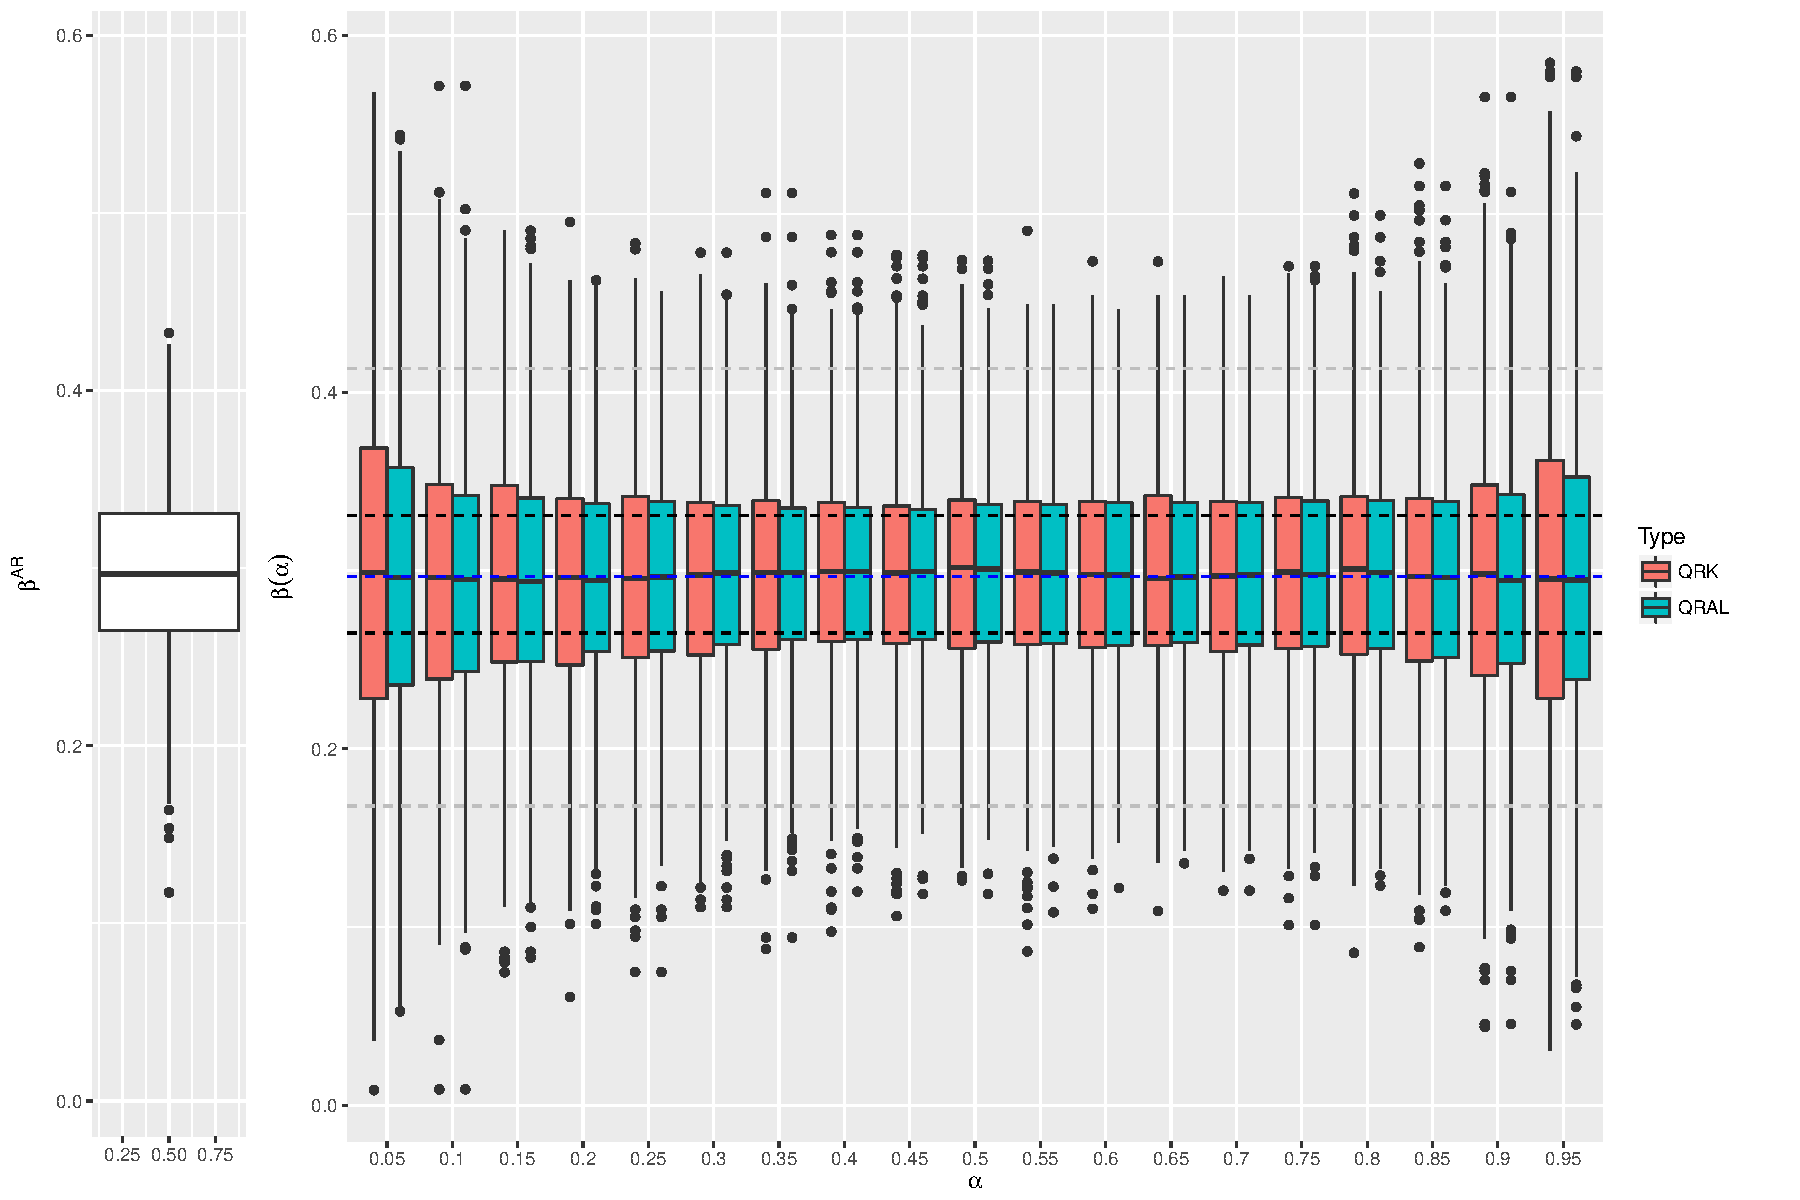
\includegraphics[width=1.0\linewidth]{Images/boxplot-ar1.pdf}
	\caption{Boxplot showing estimated coefficient after 1000 iterations. On the left hand side, the boxplot of the AR(1) coefficient estimation. Note that for the AR(1) the coefficient is equal for all probabilities $\alpha$. On the right hand side, the boxplot of the regular QR (where $\gamma = 0$) and the QRAL where $\gamma$ is selected using cross-validation. }
	\label{fig:boxplot-ar1}
\end{figure}
The conclusions from this experiment are: (i) Coefficient estimation errors for the central quantiles are not far from those estimated by the AR; (ii) extreme quantiles are usually harder to estimate, due to having fewer observations; as a consequence, the estimation error increases on the extremes (iii) QRAL has an advantage over QRK in terms of spread of estimators.


% \subsection{Controlled Studies II - Quantile autoregressive process} \label{sec:qar-study}

% In the second controlled study, the performance of QRAL is evaluated in a Quantile Autoregressive Process. While in the first study the time series $y_t$ is generated by a process with a coefficient $\beta_1$ constant across quantiles, in this experiment $\beta_1$ is a piecewise linear function of $\alpha$, described graphically on Figure \ref{fig:betas-qar}. 
% \begin{figure}[h]
% 	\centering
% 	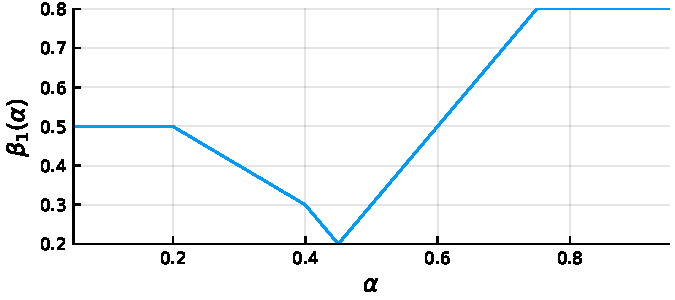
\includegraphics[width=1.0\linewidth]{Images/Betas-Qar.pdf}
% 	\caption{Coefficient $\beta_1(\alpha)$ of the autoregressive term $y_{t-1}$ for generating the QAR process.}
% 	\label{fig:betas-qar}
% \end{figure}

% The simulation of a QAR process involves two steps. The first is to determine the values of $\beta_0$ from a set of values of $\beta_1(\alpha)$; the latter given as input. These values of $\beta_{0j}$ are the output of the following optimization problem:
% \begin{IEEEeqnarray}{lr}
% 	\underset{\beta_{0}}{\text{min }} \beta_{0,|J|} - \beta_{0,1}, \span \\
% 	\text{subject to:} \span \\
% 	\beta_{0j} + \beta_{j}^T x_{t}  + h \leq \beta_{0,j+1} + \beta_{j+1}^T x_{t}, \span \nonumber  \\
% 	&\forall t \in T, \forall j \in J_{(-1)},
% \end{IEEEeqnarray}
% where $h$ is the minimum distance allowed between two neighbour quantiles. If $\beta(\alpha)$ is constant for an interval and $h$ is set to zero, this group of quantiles would superimpose one another. 
% Once both vectors $\beta_0$ and $\beta_1$ are defined, the 1-step temporal dynamic of the process can be summarized by Figure \ref{fig:qar}. 

% \begin{figure}[h]
% 	\centering
% 	\centerline{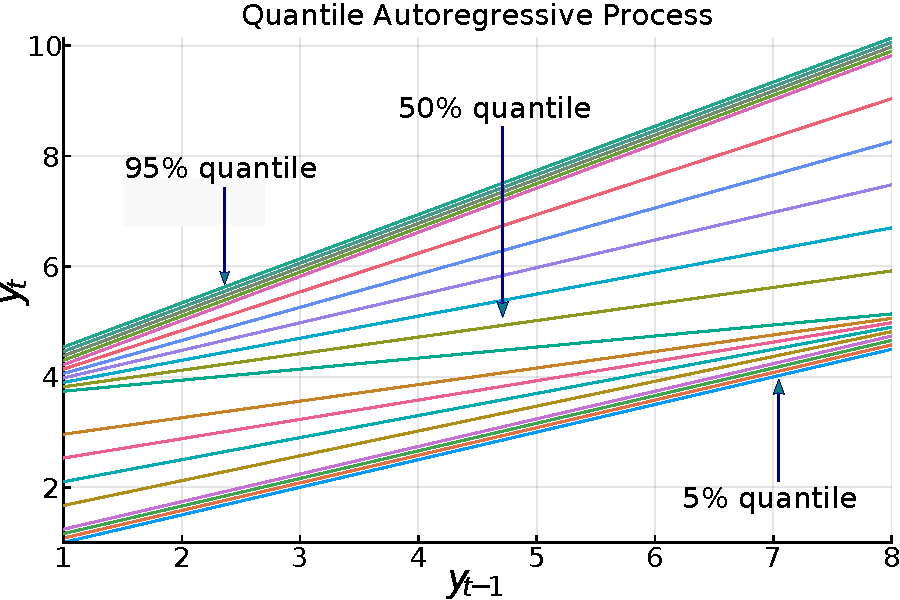
\includegraphics[width=0.8\linewidth]{Images/Qar3.pdf}}
% 	\caption{Quantiles of $y_t$ given $y_{t-1}$. For each given value of $y_{t-1}$ on the $x$-axis, the curves indicate different levels of quantiles for the values of $y_t$.}
% 	\label{fig:qar}
% \end{figure}

% The second step consists in simulating values of $y_t$. For a given value of $y_{t-1}$, the next term $y_t$ in the time series follows a distribution that can be constructed by the quantiles shown on Figure \ref{fig:qar}. 

% This controlled study has the same sample setup as the one in the previous subsection: 1000 random samples of length 400 and the same three methods tested (QRAL, QRK and AR). The objective of this experiment is to test their performance with respect to their error on the estimation of each coefficient. The summary of results is given by Table \ref{tab:qar-results}, which shows the aggregated value of quadratic error across all $j \in J$.
% The conclusion from this experiment is that both QR methods are much superior than an Autoregressive process such as a AR(1) when the coefficient $\beta$ is allowed to change with probability $\alpha$. 
% \begin{table}[h]
% \centering
% \caption{Cumulated quadratic error of coefficient estimation for each method after 1000 random samples}
% \label{tab:qar-results}
% \begin{tabular}{lll}
% \hline
% AR(1) & QRAL & QRK   \\ \hline
% 38.75 & 5.039       & 5.314
% \end{tabular}
% \end{table}

\subsection{Case Study with realistic data}

In this section, the QRAL methodology is tested in generating future scenarios of RG. A realistic time series of Wind Power is the input for estimating coefficients that are employed to generate scenarios by using the procedure described on section \ref{sec:scenario-generation}.
The time series is composed of 31 years (from 1981 to 2011) of monthly observations  of a wind farm located in the Brazilian northeast, measured in megawatts. The yearly series is shown on Figure \ref{fig:icaraizinho-mensal}.
\begin{figure}[h]
\centering
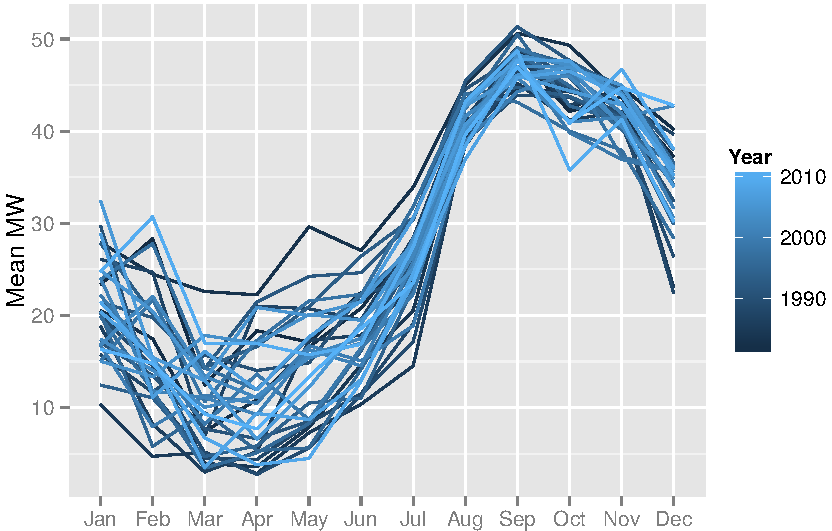
\includegraphics[width=0.8\linewidth]{Images/icaraizinho-mensal2}
\caption{Icaraizinho yearly data. Each series consists of monthly observations for each year.}
\label{fig:icaraizinho-mensal}
\end{figure}

We use four different methods to generate scenarios: QRL (Quantile Regularized LASSO, the same model as QRAL but leting $w_{ij} = 1$, for all $i$ and $j$), QRAL, QRK and SARIMA. 
The tuning parameters $\lambda$ and $\gamma$ of QRL and QRAL are selected according to two metrics: SIC and GFS.

The estimated coefficients for the QR based methods are presented on Figure \ref{fig:betas-icaraizinho}. 
\begin{figure*}[h]
	\centering
	\includegraphics[width=1.0\linewidth]{Images/Betas-icaraizinho-compilado}
	\caption{Estimated coefficients for selected quantile based methods.}
	\label{fig:betas-icaraizinho}
\end{figure*}
We show the QRAL coefficients for both SIC and GFS tuning criterias, as well as coefficients for the QRK on Figure \ref{fig:betas-icaraizinho}. For each of these methods, the coefficient $\beta_0(\alpha)$ is shown on the left panel, while the coefficients $\beta(\alpha)$ for each lag is on the right.
The biggest difference between QRK and the QRAL (SIC) is that the former presents $\beta$ coefficients which are more noisy and succeptible to variance (as seen on experiment of section \ref{sec:ar-study}), as for each quantile $j$ a completely separate problem is solved. The proposed method has the advantage that quantiles are jointly estimated in an unique model, which helps to decrease estimators variance. Regularization of covariates plays a larger role in QRAL (GFS), where fewer covariates are left nonzero.

We estimate SARIMA using the \emph{forecast} \cite{hyndman2008forecastpackage} package and the R language by using the \emph{auto.arima} function, which selects the best model according to an IC (details on \cite{hyndman2008forecastmanual}). Even though the fully automatic estimation procedure did not select seasonal differencing, we force this operation in order to produce better scenarios according to the metric GFS. The best SARIMA model is $(2,0,2)\times(2,1,0)$ with drift and seasonality of 12 periods.


The evaluation statistics for all methods are shown on Table \ref{tab:results-icaraizinho}. When comparing the performance  of QRAL and QRL, we see that for either metric the adaptive lasso produces a better estimation. 
The QRAL (SIC) performs better than QRK for both metrics, but produces worse scenarios than SARIMA. 
There is a tradeoff between having a good model for the short term (metric SIC) and having a good model for producing scenarios on the long term (metric GFS).
When choosing a metric that has a better fit for generating scenarios over one that evaluates the short term, the model must be able to select important features over the long term. On the other hand, when the model is tuned with the SIC, more variables are selected and it is able to capture better the short term fluctuations.
With selection by GFS, the size of the regularization parameters are bigger than with SIC, and the effect of bigger parameters is seen clearly on Figure \ref{fig:betas-icaraizinho} when comparing both methods, as the coefficients shrinkage is much stronger on QRAL (GFS) than in QRAL (SIC).
\begin{table}[h]
	\centering
	\caption{Cumulated statistics across all $\alpha_j$ quantiles}
	\label{tab:results-icaraizinho}
	\begin{tabular}{|l|c|c|c|c|}
		\hline 
		Method (tuning criteria) & $\lambda$ & $\gamma$ & SIC & GFS\tabularnewline
		\hline 
		\hline 
		QRL   (SIC) & 0.75 & 0.8 & 12.18 & 5.43\tabularnewline
		\hline 
		QRAL   (SIC) & 0.25 & 0.8 & 12.15 & 5.41\tabularnewline
		\hline 
		QRL    (GFS) & 9.02 & 33.1 & 13.68 & 4.58\tabularnewline
		\hline 
		QRAL   (GFS) & 1.82 & 90.01 & 13.63 & 4.23\tabularnewline
		\hline 
		QRK    ( - ) & 0 & 0 & 13.00 & 5.92 \tabularnewline
		\hline 
		SARIMA ( - ) & - & - & - & 5.15 \tabularnewline
		\hline 	
	\end{tabular}
	\end{table}
	

% The accuracy of the generated scenarios - considering the MAE metric - in recovering the historic quantiles for each month is the metric used for evaluation.

In Figure \ref{fig:simulated-quantiles}, we compare three specific quantiles (5\%, 50\% and 95\%) of the historic data with SARIMA and QRAL (with tuning by GFS) over the 12 months of the third simulated year, as explained on the section  \ref{sec:GFS} about GFS. 
\begin{figure}[h]
	\centering
	\includegraphics[width=1.0\linewidth]{Images/Comparison-scenarios-icaraizinho.pdf}
	\caption{Estimated quantiles 5\%, 50\% and 95\% of SARIMA and QRAL in comparison with historic quantiles.}
	\label{fig:simulated-quantiles}
\end{figure}
The QRAL is better in capturing the unconditional seasonality than SARIMA. It is interesting to notice that the best QRAL model according to metric GFS has fewer nonzero coefficients than the model which optimizes the SIC, but has the best results in minimizing the MAE with respect to the historic quantiles.  

